\documentclass[../book.tex]{subfiles}

\chapter{Vectorisation and its consequences}
\label{ch:vector}

\begin{quote}
The table has the function of treating multiplicity itself, distributing
it and deriving from it as many effects as possible
\autocite[149]{Foucault_1997} \index{table} \index{Foucault, Michel}
\end{quote}

\begin{quote}
We call \emph{any} set that satisfies these properties (or axioms) a
\emph{vector space}, and the objects in the set are called
\emph{vectors}. \autocite[166]{Larson_1996} \index{vector}
\index{vector space|see also {mathematics!linear algebra}}
\end{quote}

\begin{quote}
All things are vectors
\autocite[309]{Whitehead_1960}\index{Whitehead, Alfred North!on vectors}
\end{quote}

The operational power of machine learning locates data practice in an
expanding epistemic space. The space derives, I will suggest, from a
specific operational diagram that maps data into a \gls{vector space}.
It \textit{\glspl{vectorize}} data according to axes, coordinates, and
scales. Machine learning, in turn, inhabits a vectorised space, and its
operations vectorise data.
\index{data!vectorization|see {vector space!vectorization}}

Often data is represented as an homogeneous mass or a continuous flowing
stream. My aim here, however, is to archaeologically examine some of the
transformations that allow different shapes and densities of data,
whether in the form of numbers, words or images, to become machine
learnable. Data in its local complexes spaces out in many different
density shapes, depending on how the data has been generated or
instanced.\footnote{I loosely borrow the term `density' from statistics,
  where \emph{probability density functions} are often used to describe
  the hardly ever uniform distribution of probabilities of different
  values of a variable. Sensing density as a form of variation matters
  greatly both in machine learning itself, where algorithms seek
  purchase on unevenly distributed data, and in any broader diagram of
  data. Probability densities are discussed in much more detail in
  Chapters \ref{ch:probability}. The collection \emph{``Raw Data'' is an
  Oxymoron} \autocite{Gitelman_2013} evinces some of these different
  densities and distributions of data.} \index{data!density of} Whatever
the starting point -- a measuring instrument, people clicking and typing
on websites, a device like a camera, a random number generator, etc. --
machine learners only ever encounter data in specific \emph{vectorised}
shapes (vectors, matrices, arrays, etc.), mapped to a geometrically
coordinate volume. The mapping and forming, when mentioned at all, is
sometimes referred to as `data cleaning' but that term covers over
important but largely taken for granted and constitutive
transformations. \index{data!cleaning} The archaeology of data shapes
presented in this chapter explores a range of transformations focused
around the table or row-column grid. \index{archaeology!of tables}

The reshaping and re-flowing of data densities into vectors deeply
affects machine learning. This forming and reforming of data is evidence
of implicated relations. The philosopher A.N. Whitehead called `strain':

\begin{quote}
a feeling in which the forms exemplified in the datum concern
geometrical, straight, and flat loci will be called a ``strain.'' In a
strain, qualitative elements, other than the geometrical forms, express
themselves as qualities implicated in those forms
\autocite[310]{Whitehead_1960}. \index{Whitehead, A. North}
\index{data!strain}
\end{quote}

In many machine learning models the exemplified forms are straight or
flat loci (as we see in chapter \ref{ch:function}). Yet different
practices also elicit relations that strain the linear shaping of data
and these divergent relations sometimes combine in generative and
provocative ways.

\section{Vector space and geometry}\label{vector-space-and-geometry}

Statistical modelling, data-mining, pattern recognition, recommendation
systems, network modelling and machine learning rely very much on the
operation called `fitting a model.' \index{model!fitting} Fitting as a
spatial practice has some elements that resemble the phenomenologist
Edmund Husserl's account of the origin of geometry. Husserl writes:

\begin{quote}
First to be singled out from the thing-shapes are surfaces -- more or
less ``smooth,'' more or less perfect surfaces; edges, more or less
rough or fairly ``even''; in other words, more or less pure lines,
angles, more or less perfect points; then again, among the lines, for
examples, straight lines are especially preferred, and among surfaces,
the even surfaces. \ldots{} Thus the production of even surfaces and
their perfection (polishing) always plays its role in praxis
\autocite[178]{Derrida_1989}
\index{Husserl, Edmund!on thing-shapes in geometry}
\end{quote}

Husserl here refers is attempting to describe something of the way in
which forms such as planes, lines, circles, triangles, squares, and
points became objects of geometrical practice. A similar polishing and
smoothing of surfaces is certainly taking place today in the
thing-shapes we call data. The basic machine learning work of `fitting a
model' (or many models) to data is often literally implemented, as we
will see, by constraining data within a coordinate, discretized space,
which I term the \gls{\textit{vector space}} \index{vector space}

Critical thought from phenomenology to social theory has a long-standing
nervousness about the power of geometry and its gradual movement away
from shapes and things towards mathematical operations. The philosopher
Hannah Arendt, for instance, observes:

\begin{quote}
decisive is the entirely un-Platonic subjection of geometry to algebraic
treatment, which discloses the modern idea of reducing terrestrial sense
data and movements to mathematical symbols \autocite[265]{Arendt_1998}
\index{Arendt, Hannah!on geometry and algebra}
\end{quote}

The crux of the problem rests on the `treatment' or operations that
`reduce terrestrial sense data and movements' to symbols. One challenge
for contemporary thought is how to orient itself to such operations,
particularly in their data-intensive forms, without assuming that the
familiar story of scientific and technical reduction of sense and
movement to the lines and planes of modern geometry is simply reinforced
in contemporary data practice.
\index{critical thought!relation to geometry} If an archaeology of data
vectorization does anything, it needs to offer an alternative to that
reduction.

They also, as we will see, reach down into the practices of programming,
infrastructure and hardware production in ways that differ somewhat from
increases in computational power or speed. Familiar narratives of
Moore's Law increases in speed or efficiency of computation do not
account for transformations of data in \texttt{R} and other computing
environments (for instance, the popular \texttt{Map-Reduce} architecture
invented at Google Corporation to speed up its search engine services
\autocite{Mackenzie_2011} \index{data!architecture!map-reduce}).
Vectorisation transforms data along more diagrammatic lines.\footnote{Later
  chapters will discuss various ways in which the vectoral
  dimensionality of data or its rendering as \emph{vector space} scales
  up and scales down in machine learning. In terms of multiplying
  matrices, dimensionality both constrains and enables many aspects of
  the prediction. Perhaps on the grounds of data dimensionality alone,
  we should attend to dimensionality practices in \texttt{R}. A fuller
  discussion of dimensionality of data is the topic of chapter
  \ref{ch:pattern}. There I discuss how machine learning re-dimensions
  data in various ways, sometimes reducing dimensions and at other
  times, multiplying dimensions.}

\section{Mixing places}\label{mixing-places}

\begin{table}[ht]
\centering
\begingroup\tiny
\begin{tabular}{rll}
  \hline
 & Item & Title \\ 
  \hline
1 & SAheart & South African Hearth Disease Data \\ 
  2 & bone & Bone Mineral Density Data \\ 
  3 & countries & Country Dissimilarities \\ 
  4 & galaxy & Galaxy Data \\ 
  5 & marketing & Market Basket Analysis \\ 
  6 & mixture.example & Mixture Example \\ 
  7 & nci & NCI microarray data (chap 14) \\ 
  8 & orange10.test & Simulated Orange Data \\ 
  9 & orange10.train & Simulated Orange Data \\ 
  10 & orange4.test & Simulated Orange Data \\ 
  11 & orange4.train & Simulated Orange Data \\ 
  12 & ozone & Ozone Data \\ 
  13 & phoneme & Data From a Acoustic-Phonetic Continuous Speech Corpus \\ 
  14 & prostate & Prostate Cancer Data \\ 
  15 & spam & Email Spam Data \\ 
  16 & vowel.test & Vowel Recognition (Deterding data) \\ 
  17 & vowel.train & Vowel Recognition (Deterding data) \\ 
  18 & waveform.test & Simulated Waveform Data \\ 
  19 & waveform.train & Simulated Waveform Data \\ 
  20 & zip.test & Handwritten Digit Recognition Data \\ 
  21 & zip.train & Handwritten Digit Recognition Data \\ 
   \hline
\end{tabular}
\endgroup
\caption{Datasets in \textit{Elements of Statistical Learning}} 
\label{tab:datasets_elemstatlearn}
\end{table}

Data appears in \emph{Elements of Statistical Learning} in multiple
forms. \index{\textit{Elements of Statistical Learning}!datasets in}
Maps of New Zealand fishing patterns lie next to plots of factors in
South African heart disease. The 21 datasets shown in table
\ref{tab:datasets_elemstatlearn} typify the variety found in
\autocite{Hastie_2009}. They span scientific, clinical, commercial and
media fields. Note that they include many patches and pathways of
everyday life -- speaking, seeing, writing and reading -- as well as
specific scientific objects of knowledge such as galaxies, cancer,
climate and national economies. This mixture is not unusual for machine
learners. To give another example, the statistician Leo Breiman's 2001
article on random forests \autocite{Breiman_2001},
\index{machine learner!random forest} perhaps the most cited journal
paper in the machine learning literature, displays a similarly diagonal
line across human and non-human worlds: \index{Breiman, Leo}

\begin{quote}
Glass, Breast cancer, Diabetes, Sonar, Vowel, Ionosphere, Vehicle,
Soybean, German credit, Image, Ecoli, Votes, Liver, Letters, Sat-images,
Zip-code, Waveform, Twonorm, Threenorm, Ringnorm,
\autocite[12]{Breiman_2001}.
\end{quote}

In some ways, the improbable conjunction of spam email and cancer
detection in machine learning continues what statistics as a field has
always done: rove across scattered fields ranging from astronomy to
statecraft, from zoology to epidemiology, gleaning data as it goes (see
\autocites{Stigler_1986}{Hacking_1990} for samples of itineraries).
\index{statistics}

In \emph{Elements of Statistical Learning} and the field of machine
learning more generally, something more is moving through and
coordinating these datasets. The coordination might be rhetorical: the
colligation of datasets -- vowels, ozone, bone density, marketing,
prostate cancer, and spam -- in all their diversity suggests the
mobility of machine learners. The combination of datasets deriving from
network media, from medicine, from business administration and from
cutting-edge life science (c.2000) suggests a tremendous, indeed almost
spectacular miscibility, one that in principle could surprise us because
there is otherwise little mixing between the settings and knowledge
domains these datasets come from. How is this mixing, conformation and
homogenisation being done? The repetition of data sets, the
juxtaposition of discontinuous domains, and forms of movement construct
and order continuities in the service of various forms of predictive and
inferential knowledge. The miscible juxtapositions we encounter in
machine learning enter into, it seems, a \emph{regularity} or a common
space, a space that displays strong tendencies to expand, accumulate and
archive relations. Rather than peripatetic learning, the accumulation of
diverse datasets attests to a prior ordering of data to afford its
traversal.

The practices of naming and ordering, the sorting of different data
types, the addressing and expansion of data exemplified in these diverse
datasets can tell us a lot about how machine learning learns from data.
\index{learning!from data} The shapes, compositions and loci formed from
the datasets enable the functioning of machine learners as they operate
to generate statements, classifications and decisions. If machine
learning can be understood as a constantly evolving diagram of practical
abstractions, the way it draws on and relates to different forms of data
matter. As we will see, machine learners transpose data in an
increasingly extensive, heavily coordinated space, the vector space.

\section{Truth is no longer in the
table?}\label{truth-is-no-longer-in-the-table}

`This book is about learning from data' write Hastie, Tibshirani and
Friedman on the first page of \emph{Elements of Statistical Learning},
as they rapidly begin to iterate through some datasets.
\index{\textit{Elements of Statistical Learning}!on learning from data}
On the second page of the book, a table of spam email word frequencies
appears (and the problem of spam classification is canonical in the
machine learning literature - we return to in chapter
\ref{ch:probability}). \index{dataset!spam} They come from the dataset
\texttt{spam} \autocite{Cranor_1998}. On the third page, a complicated
data graphic appears (Figure 1.1, \autocite[3]{Hastie_2009}. It is a
scatterplot matrix of the \texttt{prostate} dataset included in the
\texttt{R} package \texttt{ElemStatLearn,} the companion \texttt{R}
package for the book. In a third example, a set of scanned handwritten
numbers appears. These scans are images of zipcode or postcode numbers
written on postal envelopes taken from the dataset \texttt{zip}
\autocite{LeCun_2012}, and they differ from both the \texttt{spam} table
and \texttt{prostate} plots because they directly resemble something in
the world, which, however, happens to be numbers, and is, therefore,
probably already recruited into data-making and data-circulating
processes (a dataset we return to in chapter
\ref{ch:subjects}).\index{dataset!\texttt{zip}} The final example in the
introduction, `Example 4: DNA Expression Microarrays,' draws from
biology, and particularly, high-throughput genomic biology, a science
that produces large amounts of data about biological processes by
running many tests, or by constructing devices that generate many
measurements, in this case, a DNA microarray.\footnote{Some genomic data
  will be the focus of a later chapter \ref{ch:genome}. Machine learning
  during the 1990s and 2000s was in some ways boosted heavily by the
  advent of genomic biology with its large, enterprise style knowledge
  endeavours such as the Human Genome Project.}

The table or the row-column addressable grid is common to all of these
datasets. And yet, as we are about to see, machine learning in many ways
deals with the collapse or liquidation of tabular datasets. `Things, in
their fundamental truth,' writes Foucault in \emph{The Order of Things}
`have now escaped from the space of the table'
\autocite[239]{Foucault_1992}. \index{Foucault, Michel!on table}
\index{table!history |(} Foucault writes in these pages about the fabled
emergence of life, labour and language as the anchoring vertexes of a
new triangle of knowledge and power structuring the figure of the
`human' in the 19th century.

Before the emergence of the characteristic sciences of the human --
political economy, linguistics and biology -- knowledges such as natural
history, the general grammars, and philosophies of wealth (such as Adam
Smith's work) had ordered empirical materials of diverse provenance in
tables or grids. While the history of tables as data forms reaches a
long way back (see \autocite{Marchese_2013} for a broad historical
overview that reaches back to Mesopotamia), Foucault argues that the
Classical age first developed the system of grids that permitted
ranking, sorting and ordering in tables. These grids replace the
Renaissance tabulations based on `buried similitudes' and `invisible
analogies' \autocite[26]{Foucault_1992}. In pre-Classical tables, an
image or figure from myth might lie alongside a measurement or a count
of occurrences, and this proximity was ordered by systems of analogical
association that spanned what we might today, in the wake of the 19th
century, might see as incongruous (for instance, associations between
medicine and Biblical prophecy).

The Classical Age grid or table, by contrast, brought plural and diverse
resemblances into exhaustive systematic visible enumeration. As Foucault
puts it:

\begin{quote}
The space of order, which served as a \emph{common place} for
representation and for things, for empirical visibility and for the
essential rules, which united the regularities of nature and the
resemblances of imagination in the grid of identities and differences,
which displayed the empirical sequence of representations in a
simultaneous table, and made it possible to scan step by step, in
accordance with a logical sequence, the totality of nature's elements
thus rendered contemporaneous with one another
\autocite[239]{Foucault_1972}
\end{quote}

The table as space of order did not stand in isolation. It served a
localized epistemic function in conjunction with other of knowledge such
as experiment and mathematical proof. Since algebra or experimental
\emph{mathesis} only applied to `simple natures' (planets in movement,
dynamics of falling bodies, etc.),
\index{mathematics!application to nature} table-based knowledges such as
taxonomy dealt with more complex natures. In the tables, systems of
signs -- for instance, the groupings established by the eighteenth
century taxonomist Carl Linnaeus -- sought to reduce complex natures
(plants, animals, etc.) to simpler forms as columns and rows in a table
based on resemblances and similarities. \index{Linnaeus, Carl}
\index{differences!taxonomy of} Importantly, the table as space of order
was a space of imagination in that one could begin to see continuities
and differences between things (organisms, words, nations) by carefully
ordering and scanning the table. `Hedged in by calculus and genesis,'
Foucault suggest, `we have the area of the \emph{table}'
\autocite[73]{Foucault_1992}. \index{calculus|see{mathematics!calculus}}
Note in passing that calculus and calculations bound the table only in
relation to `simple natures' whose identity and difference can be
understood in the form of movements, rates and change in
position.\footnote{In \emph{Surveiller et Punir} or \emph{Discipline and
  Punish} \autocite{Foucault_1977}, Foucault returned to the question of
  the table in a slightly different context: an account of the operation
  of power in disciplinary institutions and knowledges. In these
  knowledges, the table becomes generative of `as many effects as
  possible.' \index{Foucault, Michel!tables!in disciplinary power}} This
is an important limitation since it is precisely the complex natures in
genesis that machine learning tries to engage using algebra, calculus,
statistics and computation.

Finally (at least for our purposes), in the nineteenth century, a
different form of ordering shattered tabulation based on enumerated
similarity and ordered resemblance. Foucault figures this change as
shattering the table into shards of order:

\begin{quote}
this space of order is from now on shattered: there will be things, with
their own organic structures, their hidden veins, the spaces that
articulates them, the time that produces them; and then representation,
a purely temporal succession, in which those things address themselves
(always partially) to a subjectivity \autocite[239-240]{Foucault_1992}.
\end{quote}

Life, labour and language -- Foucault's famous historically emergent
triadic figure of the human -- replace the enumerative, synoptic
classificatory tables of the Classical age. Tables still abound in newer
temporal, genetic orderings (almost any episode from the history of
nineteenth and twentieth century statistics will confirm that; see
\autocites{Stigler_1986}{Stigler_2002})\index{statistics!history}, but
from now on tables are localized, relating to a place and changing in
time, and functioning as shards of representational order addressed to
(and often constitutive) of subject position.
\index{subject position!human!historical constitution of} A double
interiority takes over. Things such as a language, a species or an
economic system have their own genesis, their own temporality and
historical existence. Our knowledges and indeed experience of them also
become finite, historical, with their own dynamics and internal life. In
this change, the table itself is no longer the foundation or
distillation of knowledge. It is one knowledge apparatus amongst many.
\index{table!history|)} Tables, we might say, become merely data,
inscriptions pendant on hidden structures and their genesis.
\index{data!tables become}

This brief résumé of a thread of argument in \emph{The Order of Things}
might help us reassess how machine learning goes into the data. The
tables of \texttt{spam}, \texttt{prostate}, \texttt{image} and
\texttt{microarray} data in contemporary machine learning do not operate
in the way Linnaeus would have tabulated a table of living things based
on similarities and resemblances or a Renaissance medical textbook might
assemble analogical resemblances between disease and astronomy. As I
will argue, measures of similarity and resemblance still operate
strongly in machine learning as it moves through tables. In this
respect, the Classical table and perhaps even the pre-Classical table
returns with extended relevance. The repeated juxtaposition of tables of
diverse provenance alongside each other, the incorporation of `complex
natures,' and the operational superimposition of different tables
suggests machine learners still suggest synoptic alignments, but along
different lines than the row-column grid of the Renaissance, Classical
or even the later life-labour-language tables of the human sciences.
Even if the tables in the opening pages of \emph{Elements of Statistical
Learning} concern work, life, language and economy and map very readily
onto the anchor points, the new `empiricities' (Foucault's term for the
empirical problems), of labour, life and language or biopower
\index{biopower} that took root at this time \autocite{Foucault_1991},
the ways machine learners traverse them may not be recognisable in terms
of these empiricities. \index{empiricities}

Instead, we are now confronted by kaleidoscopically transmuted tables
whose expansion and open margins afford many formulations of similarity
and difference. Already in the handwritten digits and the microarray
data, scale and dimensions thwart tabular display of the data. In
settings such as social media platforms or genomics in which machine
learning operates, tables change rapidly in scale and sometimes in
organisation. The multiplication and juxtaposition of tables suggests
that we might be seeing the advent of a post-order space for
regularities and resemblances, for simple and complex natures,
encompassing knowledges ranging from humanities to traffic engineering.

\section{The epistopic fault line in
tables}\label{the-epistopic-fault-line-in-tables}

The \texttt{ElemStatLearn} \texttt{R} package brings, as we have seen in
the previous chapter, with it around 20 different datasets, including
the four mentioned in the introduction to \emph{Elements of Statistical
Learning}. On the one hand, every data table indexes a localised complex
of activities (clinical research, social media platform, financial
transactions, etc.) with possible referential
importance.\index{referentiality} On the other hand, for machine
learners, the table is a space of potential similarities and differences
both internal to the table itself (e.g.~how much does row number 1000
differ from row 1,000,000) and associated with other tables (e.g.~how
much does this table of clinical test relate to that table of microarray
data?). \index{differences!between datasets} These internal and external
differences entwine with each other in ways that create a fault line, an
unstable yet generative line of diagonal movement. It is this fault or
fold line, I propose, that diagrammatically distributes data tables into
the expansive and moving substrata of the vector space.
\index{diagrammatic movement}

The table has been vectorised. We might say that the vectorization of
the table is epistopic. The term `epistopic' \index{epistopic} comes
from the work of the science studies scholar Mike Lynch
\index{Lynch, Mike!epistopics} whose account of scientific practice is
particularly focused on ordinariness\index{practice!scientific}. Akin to
what Foucault in the \emph{Archaeology of Knowledge} terms a threshold
of epistemologization \autocite[195]{Foucault_1972}
\index{epistemologization!threshold of} Lynch characterizes the
`epistopic' as connecting localized practices (`topics') with `familiar
themes from epistemology and general methodology' in the local
achievement of coherence in knowledge \autocite[280]{Lynch_1993}.
\index{knowledge!local coherence of} In other words, as the term itself
suggests, an epistopic connects general epistemic themes such as
validity, precision, specificity, error, confidence, expectation,
likelihood, uncertainty, or approximation with a place, a `local complex
of activities' (281). \index{machine learning!statistical aspects} This
emphasis on epistemic location frames the problem of how the `local
complex' of a specific dataset encounters a generalizing epistemic
practice such as machine learning. \index{epistemology}

\section{Surface and depths: the problem of volume in
data}\label{surface-and-depths-the-problem-of-volume-in-data}

The local complex of activities for associating datasets shatters tables
from a different direction than that described by Foucault in \emph{The
Order of Things}. Algebra, linear algebra in particular, organizes and
distributes differences in vector space. \emph{Mathesis} in the form of
algebraic operations of addition and multiplication of collections of
tabular elements such as rows and columns, now re-defined as vectors,
re-structure tabular data as a vector space, as a `set' whose membership
is only limited by the applicability of the constructing relations.
These operations absorb and subtend differences in quality, type, kind
and quantity. \index{vector space!ramification in}

\begin{table}[ht]
\centering
\begingroup\tiny
\begin{tabular}{rrrrrrrrrrl}
  \hline
 & lcavol & lweight & age & lbph & svi & lcp & gleason & pgg45 & lpsa & train \\ 
  \hline
1 & -0.58 & 2.77 &  50 & -1.39 &   0 & -1.39 &   6 &   0 & -0.43 & TRUE \\ 
  2 & -0.99 & 3.32 &  58 & -1.39 &   0 & -1.39 &   6 &   0 & -0.16 & TRUE \\ 
  3 & -0.51 & 2.69 &  74 & -1.39 &   0 & -1.39 &   7 &  20 & -0.16 & TRUE \\ 
   \hline
\end{tabular}
\endgroup
\caption{First rows of the `prostate` dataset} 
\label{tab:prostate}
\end{table}

\begin{figure}
  \centering
      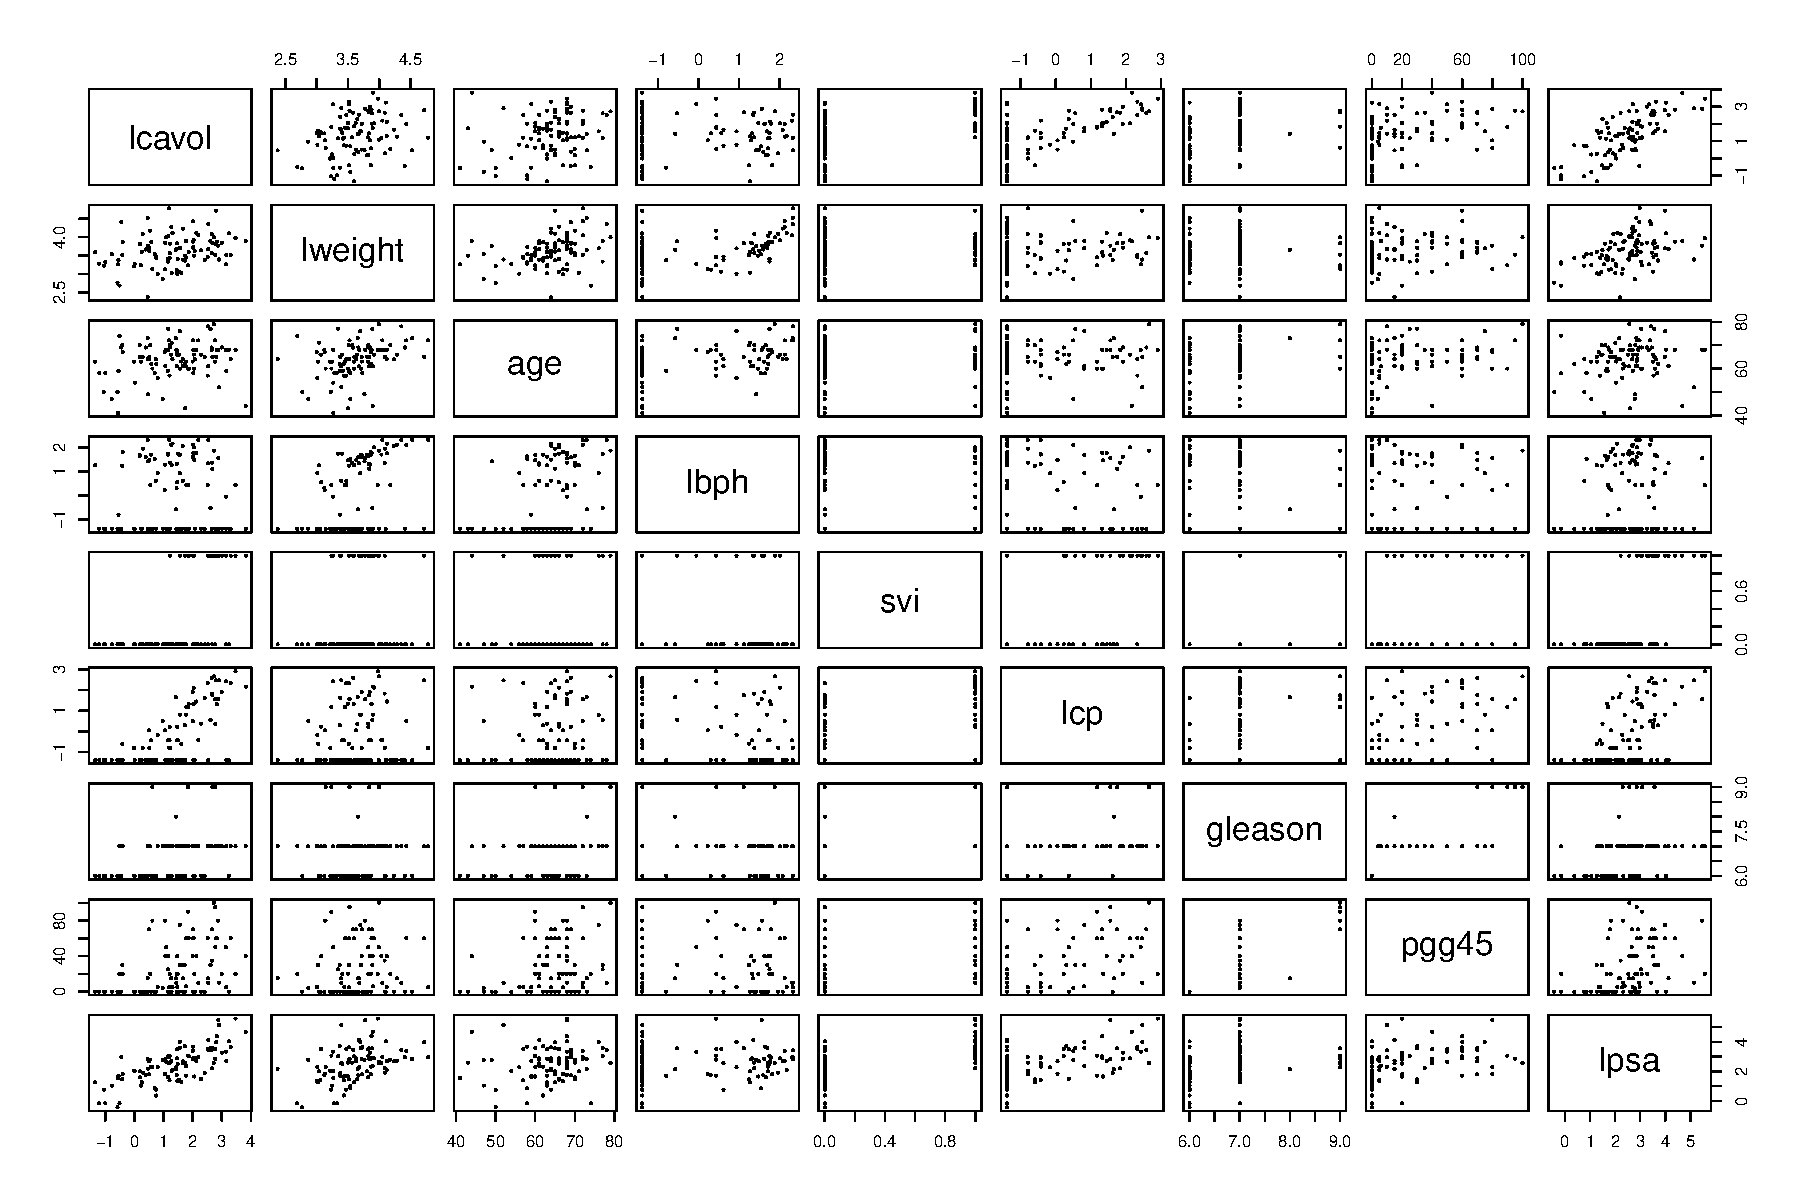
\includegraphics[width=0.9\textwidth]{figure/prostate_plot-1.pdf}
        \caption{Scatter plot matrix of \texttt{prostate} data}
  \label{fig:prostate_plot_matrix}
\end{figure}

Of the three example datasets (\texttt{prostate}, \texttt{spam} and
\texttt{zip}), \emph{Elements of Statistical Learning} returns most
frequently to \texttt{prostate.} This dataset derives from the work of
urologists working at Stanford \autocite{Stamey_1989}, and concerns
various clinical measurements performed on men who were about to undergo
radical prostatectomy. The measurements range across the volume and
weight of the prostate, as well as levels of various prostate-related
biomarkers such as PSA -- prostate specific antigen. Several rows from
the dataset are shown in Table \ref{tab:prostate}. The first pages of
the book had already exhaustively plotted all the variables in the
dataset against each other using the table-related form of a scatter
plot matrix \autocite[3]{Hastie_2009} (shown in figure
\ref{fig:prostate_plot_matrix}, and they return to the same data on
almost a dozen occasions in the course of the book, subjecting it to
repeated vectorization. \index{dataset!prostate}
\index{graphic!scatterplot matrix}

The contrast between the Table \ref{tab:prostate} and the Figure
\ref{fig:prostate_plot_matrix} already depends on a transformation
intrinsic to vectorization. On the one hand, the table arrays all
different data types in rows and columns. In the table, the relation
between the different data types (the log of the weight of prostate -
\texttt{lwp} and \texttt{age} for instance) is quite hard to see.
Moreover, different kinds of variables stand side by side. \texttt{svi},
short for `seminal vesicle invasion' is a categorical variable.
\index{data!type!categorical} It takes the values `true' or `false,'
shown here as \texttt{1} or \texttt{0}, but the other variables either
measure or count things (years, sizes, or levels of antigens).

On the other hand, the scatter plot matrix also takes the form of a
grid-like figure, but the cells of the grid are not occupied by numbers
but by \texttt{x-y} plots of different pairs of variables in the
\texttt{prostate} dataset. The `matrix' of figures shows of 72 plots is
mirrored across the diagonal that runs from the top-life to bottom right
in figure \ref{fig:prostate_plot_matrix}. Taking this folding into
account, we see 36 unique plots with different data in each one. Each
sub-plot displays the relation between two variables in the dataset as a
scatter plot. Some variables such as \texttt{svi} are not very amenable
to plotting in this way. More importantly perhaps, certain combinations
of variables appear as flat loci that can be read as signs of relations
between different variables. The scatter plot matrix constructs a
tabular space in which relational contrasts between pairs of variables
start to appear. In the light of these contrasts (and I use `light' here
in an almost literal sense to refer to the way in which the architecture
of the figure creates a space in which light scatters in varying
patterns), the \texttt{prostate} dataset begins to expose relations that
might be worth knowing about. We have moved on from the bare table of
the dataset to a transformed tabulation, from a textual-numerical grid
to a geometrical-numerical grid. Everything remains on the surface of a
grid here, but the grid permits differences in relationality to begin to
appear. \index{differences!visibility in data}

All of this somewhat precedes the operational formation of machine
learning. Similar tables and plots are part and parcel of statistical
data exploration more generally (see \autocite{Beniger_1978} for an
historical account of quantitative graphics in statistics).
\index{statistics!graphics| seealso {graphics}} The scatterplot matrix
does not exhaust differences or relationality in the \texttt{prostate}
dataset, but highlights a tendency to approach it from different angles
(12 times in the \emph{Elements of Statistical Learning}) in order to
map the multiple relations or influences that remain opaque to even the
most exhaustive matrices of plots. The scatterplot matrix shows pairs of
variables in relation. If the crucial diagnostic factor in this case is
an elevated level of the PSA (prostate specific antigen), how do we know
what combinations of other measurements might be associated with its
elevation? What if multiple variables affect the level of PSA?\footnote{Despite
  the intensive work that Hastie and co-authors conduct on the
  \texttt{prostate} data, all with a view to better predicting PSA
  levels using volumes and weights of prostates, etc., Stamey and other
  urologists more than a decade or so concluded that PSA is not a good
  biomarker for prostate cancer. \index{dataset!prostate} Stamey writes
  in 2004:

  What is urgently needed is a serum marker for prostate cancer that is
  truly proportional to the volume and grade of this ubiquitous cancer,
  and solid observations on who should and should not be treated which
  will surely require randomized trials once such a marker is available.
  Since there is no such marker for any other organ confined cancer,
  little is likely to change the current state of overdiagnosis (and
  over-treatment) of prostate cancer, a cancer we all get if we live
  long enough. \autocite[1301]{Stamey_2004}} This question can just
about be pursued by scanning the matrix of plots, but not very stably
since different data analysts might see different associations combining
with each other there. Different statements or epistopics could be
supported by the same figure. \index{statements!epistopic elements of}

The very question of relation between multiple variables and the
predicted levels of PSA suggests the existence of a hidden, occluded or
internal space that cannot be seen in a data table, and that cannot be
brought to light even in the more complex geometry of a plot. This
volume contains the locus of multiple relations, a locus inhering in a
higher dimensional space, in this case, the nine dimensional space
subtended by treating each of the nine variables or columns in the
\texttt{prostate} dataset as occupying its own dimension. A different
basis of order -- the vector space -- \index{vector space|(} begins to
take shape when dataset variables (usually columns in a table) become
dimensions.\footnote{Every distinct column in a table practically adds a
  new dimension to the vector space. Since the 1950s, problems of
  classification and prediction in high-dimensional spaces have been the
  object of mathematical interest. The mathematician Richard Bellman
  coined the term `the curse of dimensionality' to describe how
  partitioning becomes more unstable as the dimensions of the space
  increase \autocite{Bellman_1961}.
  \index{Bellman, Richard!curse of dimensionality} The problem is that
  while the volume of a space increases exponentially with dimensions,
  the number of data points (actual measurements or observations)
  usually does not usually increase at the same rate. In high
  dimensional spaces, the data becomes more thinly spread out. It is
  hard to partitions sparsely populated spaces because they accommodate
  many different boundaries.
  \index{vector space!dimensionality!curse of}}

\section{Vector space expansion}\label{vector-space-expansion}

To show how this space opens up, we might follow what happens to just
one or two columns of the \texttt{prostate} data in the vector space as
it is vectorized. \index{vectorization!of data} In the \texttt{prostate}
dataset, some variables are continuous quantitative values, some are
categorical (they represent membership in a group or category) and some
are ordinal variables (they represent a ranking or order).
\index{data!type!continuous} \index{data!type!ordinal}
\index{data!type!categorical} How can different data types be located in
vector space? In order to put classifications or categories into vector
space, they need to be translated into the same \emph{basis} as the
quantitative variables with their rather more obvious geometrical and
linear coordinate values. \index{vector space!basis of} How does one
geometrically or indeed algebraically render a category or a qualitative
difference? The problem is solved via an expansion of the vector space
through a form of binary coding that generates a new variable and hence
a new dimension for each category:

\begin{quote}
Qualitative variables are typically represented numerically by codes.
The easiest case is when there are only two classes or categories, such
as ``success'' or ``failure,'' ``survived'' or ``died.'' These are often
represented by a single binary digit or bit as 0 or 1, or else by 1 and
1 \ldots{} When there are more than two categories, several alternatives
are available. The most useful and commonly used coding is via dummy
variables. Here a K-level qualitative variable is represented by a
vector of K binary variables or bits, only one of which is ``on'' at a
time \autocite[12]{Hastie_2009} \index{data!type!categorical!coding of}
\end{quote}

Again, the details are not so important here as the transformations that
the vector space accommodates. A single qualitative or categorical
variable expands into `a vector of K binary variables or bits.'
Qualitative data, once coded in this way, can be multiplied, added, and
in short, handled algebraically using the same aggregate operations
applied to numerical or continuous variables. Not only has the vector
space expanded here, its expansion smooths over important fault-lines of
difference that vertically divided the tabular data. Complex natures
become simple natures. The different kinds of variables -- qualitative
and quantitative, discrete and continuous, nominal and ordinal -- can be
accommodated by adding dimensions to the vector space.
\index{vector space|)} As Whitehead says, `all things are vectors'
\autocite[309]{Whitehead_1960}

Adding dimensions to vector space subsumes differences, but makes seeing
the geometrically regular loci -- lines, planes, smooth surfaces -- in
data distributed in this space more challenging. The many
transformations in \texttt{prostate} that ensue in \emph{Elements of
Statistical Learning} become the locus of machine learning.
\index{machine learning!epistopic} In a historically significant
transfiguration of the table, these expansions -- and we will see
others, including \emph{de novo} creations of constructed dimensions --
subtend differences in a vector space comprising elements defined purely
by coordinate position and vectoral (having direction and extent)
movement. \index{vector space!dimension} Once this hidden, expandable
and transformable (by rotation, displacement, or scaling) distribution
of elements in space exists, strenuous efforts will be made to bring
loci to light. Machine learners search for these loci or or feel for
\glspl{data strains}, to use Whitehead's term, \index{data!strain} along
different lines. Sometimes a machine learner prehends vector space as
filled with constantly varying proximities. It gathers and orders these
proximities (for instance, as in the \emph{k} nearest neighbours model
\index{machine learner!\textit{k}-nearest neighbours model}) or in
unsupervised methods such as k-means clustering
\autocite[513]{Hastie_2009}\index{machine learner!\textit{k}-means clustering}.
More commonly, machine learning draws lines or flat surfaces that
con-strain the volume. \index{vector space!strain}

\index{machine learner!linear regression model} The importance of lines
and flat surfaces can hardly be under-estimated in machine learning.
Finding lines of best fit underpins many of the machine learners that
attract more attention (neural nets, support vector machines, random
forests). Linear regression with its pursuit of the straight line or
plane projects the basic alignments of vector space. It renders all
differences as distances and directions of movement. Drawing lines or
flat surfaces at various angles and directions is perhaps the main way
in which the volume of data is traversed, and a relation between input
and output, between predictors and prediction, consolidated as a loci or
data strain loci or data strain.\footnote{One sign of the centrality of
  the line in machine learning can be seen, for instance, from the
  contents page of the book \autocite[xiii-xxii]{Hastie_2009}. After the
  introduction of the linear model in the first chapter and its initial
  exposition in chapter 2 (`overview of supervised learning'), it forms
  the central topics of chapter 3 (`linear methods for regression'),
  chapter 4 (`linear methods for classification'), chapter 5 (`basis
  expansions and regularization'), chapter 6 (`kernel smoothing
  methods'), much of chapter 7 (`model assessment and selection'),
  chapter 8 (`model inference and averaging'), major parts of chapter 9
  (`additive models, trees and related methods'), important parts of
  chapter 11 (`neural networks' -- neural networks can be understood as
  a kind of regression model), the anchoring point of chapter 12
  (`support vector machines and flexible discriminants') and the main
  focus in the final chapter (`high dimensional problems'). A similar
  topic distribution can be found in Andrew Ng's Cs229 lectures on
  machine learning. More than half of the 20 lectures concern linear
  models and their variants. See
  \autocites{Ng_2008a}{Ng_2008b}{Ng_2008c}{Ng_2008d}.} The line of best
fit has a ready generalization to higher dimensions, and a line can be
diagrammed in the equations of linear algebra, the field of mathematics
that operates on lines in spaces of arbitrary dimensions.
\index{linear algebra|(} Linear algebra operations exist for finding
intersections between lines and planes, for manipulating collections of
elements and aggregate forms such matrices \index{data!matrix as}
through mappings and transformations (rotations, displacements or
translations, skewing, and scaling), and above all, handling whole
vector spaces as operational sets. It brings with it a set of
formalisations -- vector space, dimension, matrix, determinant,
coordinate system, linear independence, eigenvectors and eigenvalues,
inner-product space, etc. -- that machine learners constantly and
implicitly resort to invoke.\footnote{Along with statistics and
  probability, linear algebra is a such an important part of machine
  learning that many books and courses recommend students complete a
  linear algebra course before they study machine learning. Cathy
  O'Neill and Rachel Schutt advise: When you're developing your skill
  set as a data scientist, certain foundational pieces need to be in
  place first---statistics, linear algebra, some programming
  \autocite[17]{Schutt_2013}}
\index{machine learning!reliance on linear algebra}

Many of these operations quickly become difficult to geometrically
figure. \footnote{We might add also approach the epistopic fault line in
  machine learning topologically \index{topology}. Over a decade ago,
  the cultural theorist Brian Massumi wrote that `the space of
  experience is really, literally, physically a topological hyperspace
  of transformation' \autocite[184]{Massumi_2002}
  \index{Massumi, Brian}. Much earlier, Gilles Deleuze had
  conceptualised Michel Foucault's philosophy as a topology, or `thought
  of the outside' \autocite{Deleuze_1988}, as a set of movements that
  sought to map the diagrams that generated a `kind of reality, a new
  model of truth' \autocite[35]{Deleuze_1988}. More recently, this
  topological thinking has been extended and developed by Celia Lury
  amongst others. In `The Becoming Topological of Culture,' Lury,
  Luciana Parisi and Tiziana Terranova suggests that `a new rationality
  is emerging: the moving ratio of a topological culture'
  \autocite[4]{Lury_2012} \index{Lury, Celia}. \index{Parisi, Luciana}
  \index{Terranova, Tiziana} In this new rationality, practices of
  ordering, modelling, networking and mapping co-constitute culture,
  technology and science \autocite[5]{Lury_2012}. At the core of this
  new rationality, however, lies a new ordering of continuity. The
  `ordering of continuity,' Lury, Parisi and Terranova propose, takes
  shape `in practices of sorting, naming, numbering, comparing, listing,
  and calculating' (4). The phrase `ordering of continuity' is
  interesting, since we don't normally think of continuities as subject
  to ordering. In many ways, that which is continuous bears within it
  its own ordering, its own immanent seriation or lamination. But in the
  becoming topological of culture, movement itself undergoes a
  transformation according to these authors. Rather than movement as
  something moving from place to place relatively unchanged (as in
  geometrical translation), movement should be understood as more like
  an animation, a set of shape-changing operations. These
  transformations, I would suggest, should be legible in the way that
  machine learning, almost the epitome of the processes of modelling and
  calculation that Lury, Parisi and Terranova point to, itself moves
  through the data. And indeed, the juxtaposition of spam, biomedical
  data, gene expression data and handwritten digits already suggests
  that topological equivalences, and a `radical expansion' of comparison
  might be occurring. Bringing epistopics and topologies together might,
  I suggest, help trace, map and importantly diagram some of the
  movements into the data occurring today.} Let us return to the
equations for linear regression models (remembering that both C.S.
Pierce and Andrew Ng advocate returning often to equations). The
`mainstay of statistics,' the linear regression model, usually appears
diagrammatically in a more or less algebraic form:

\begin {equation}
\label {eq:linear_model}
\hat{Y}=\hat{\beta_0}  + \sum^p_{j=1}X_j\hat{\beta_j}
\end {equation}

\begin {equation}
\label {eq:linear_model_vector}
\hat{Y} = X_T\hat{\beta}
\end {equation}

Equations \ref{eq:linear_model} and \ref{eq:linear_model_vector} express
a plane (or hyperplane) in increasingly diagrammatic abstraction. The
possibility of diagramming a high dimensional space derives largely from
linear algebra. Reading Equation \ref{eq:linear_model} from left to
right, the expression \(\hat{Y}\) already points to a set of calculated,
predicted values, or a vector of \(y\) values, such as all the
\texttt{lpsa} or PSA readings included in the \texttt{prostate} dataset.
Similarly, the term \(X_j\) points to the table of all the other
variables in the \texttt{prostate} dataset. \index{dataset!prostate}
Since there are 8 other variables, and close to 100 rows, \(X\) is a
\emph{matrix} -- a higher dimensional table -- of values, addressable by
coordinates. \index{mathematics!linear algebra!matrix} Finally
\(\beta_j\) are the pivotal coefficients or multiplying quantities that
determine the slope or direction of the lines drawn.
\index{deep learning} The second expression Equation
\ref{eq:linear_model_vector} relies more fully on linear algebra. This
is the linear model written in `vector form' \autocite[11]{Hastie_2009},
or vectorized. The right hand side comprises two operations \(X^T\), the
transpose or rotation of the data, and implicitly -- multiplication is
hardly ever shown, but diagrammed by putting terms alongside each other
-- an \emph{inner product} of the \(X\) matrix and the \(\beta\)
parameters (to use model talk) or coefficients (to use linear algebra
talk). \index{parameters|seealso{model!coefficient}}\footnote{Carl
  Friedrich Gauss \index{Gauss, Carl Friedrich} and Adrien-Marie
  Legendre's work on linear regression at this time is well-known. The
  first independent use of linear regression was Gauss' prediction of
  the location of an `occluded volume,' the position of the asteroid
  Ceres after it reappeared in its orbit behind the sun.
  \autocite{Stigler_2002} -- TBA page ref}
\index{mathematics!linear algebra!dot or inner product}

The vector form in equation \ref{eq:linear_model} diagrams an inclined
plane that cannot be fully drawn in any figure, only projected
perspectivally onto the surface of a graphic plot. While that line can
never fully come to light, the diagrammatics of equations
\ref{eq:linear_model} and \ref{eq:linear_model_vector} express a way of
constructing it and orienting it in vector space. Such expressions are
epistopic in that they connect the local complex of activities indexed
as tabulated data together through the diagonal diagrammatic element of
a line or plane angling through vector space.

\section{Drawing lines in a common space of
transformation}\label{drawing-lines-in-a-common-space-of-transformation}

\begin{figure}
  \centering
      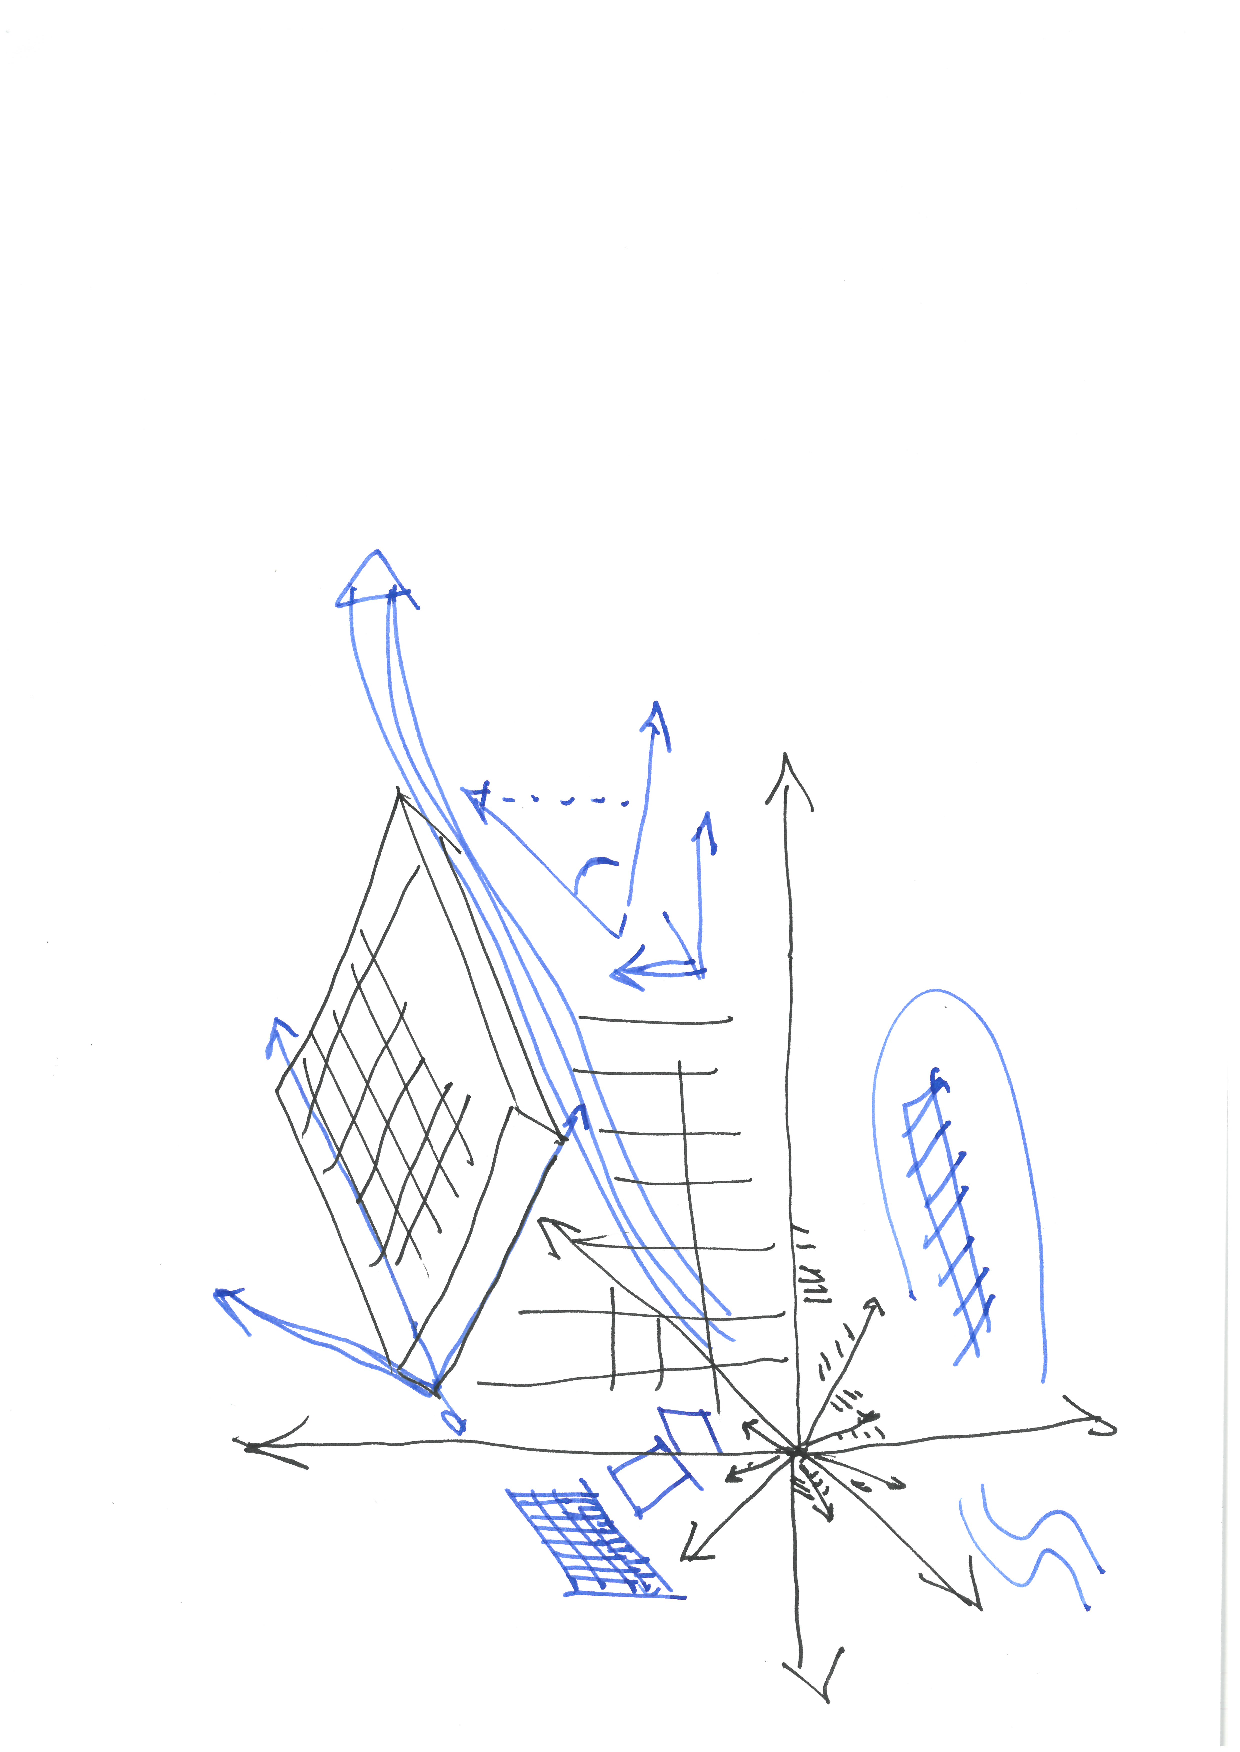
\includegraphics[width=0.5\textwidth]{figure/vector_space.png}
        \caption{Vector space comprises transformations}
  \label{fig:common_space}
\end{figure}

Once data is distributed in vector space, machine learners operate as
transformations of that space into other vector spaces, the flat loci.
Indeed from the perspective of vector space, machine learners are simple
transformations or operations that map vector spaces into different
ones, usually of lower but sometimes of higher dimensionality.
\index{machine learning!as transformation of vector space} For instance,
`drawing' the line of best fit through the \texttt{prostate} data or
`fitting a line' can be understood as a purely algebraic operation
(although in practice, most machine learners are not purely algebraic --
they optimise and probabilise, as we will see). \index{linear algebra|)}
Viewed in terms of linear algebra, the analytical or `closed form
solution' for the parameters of the linear model is given in equation
\ref{eq:linear_model_solution}: \index{model!fitting of}
\index{machine learner!linear regression!closed form solution to}

\begin {equation}
\label {eq:linear_model_solution}
\hat{\beta} = (\mathbf{X}^T\mathbf{X})^-1\mathbf{X}^T\mathbf{y}
\end {equation}

In this expression, linear algebraic operations on the data shown as
\(\mathbf{X}\) calculate the coefficients \(\hat{\beta}\) that orient a
plane cutting through the vector space.\footnote{Perhaps more
  importantly, the linear algebraic expression of these operations
  presupposes that all the data, both the values used to build the model
  and the predicted values the model may generate as it is refined or
  put into operation somewhere, are contained in a common space, the
  vector space, a space whose formation and transformation can be
  progressively ramified and reiterated by various lines that either
  separate volumes in the space, or head in a direction that brings
  along most of the data. Not all of these lines are bound to be
  straight, and much of the variety and dispersion visible in machine
  learning techniques comes from efforts to construct different kinds of
  lines or different kinds of `decision boundaries' (in the case of
  classification problems) in vector space (for instance, the k-nearest
  neighbors method does not construct straight lines, but somewhat
  meandering curves that weave between nearby vectors in the vector
  space; see \autocite[14-16]{Hastie_2009}).
  \index{machine learner!\textit{k}-nearest neighbours} Whether they are
  straight or not, the epistopic aspect of these lines remains
  prominent. Typically, many different statistical tests (Z-scores or
  standard errors, F-tests, confidence intervals, and then prediction
  errors) will be applied to any estimate of the coefficients of even
  the basic linear regression model, well before most advanced or
  sophisticated models and techniques (cross-validation, bootstrap
  testing, subset and shrinkage selection) begin to re-configure the
  model in more radical ways. \index{statistics!tests}} The derivation
of the analytical `ordinary least squares' solution
\index{machine learner!linear regression!ordinary least squares} relies
on some differential calculus \index{mathematics!calculus!differential}
as well as a range of linear algebra operations such as matrix
transpose, inner product and matrix inversion, the details of which need
not trouble us here. The relevant point is that equation
\ref{eq:linear_model_solution} constructs a plane -- a new vector --
that traverses the density-shape of a dataset in its full dimensional
vector space (nine dimensions in the case of
\texttt{prostate}).\footnote{As we will see in the following chapter
  (chapter \ref{ch:function}), it is not always possible to calculate
  the parameters of a model analytically. Especially in relation to
  contemporary datasets that have very many variables and many instances
  (rows in the table), linear algebra approaches become unwieldy in
  their attempt to produce exact results, and machine learning steps in
  with a variety of computational optimisation techniques.
  \index{coefficients}}

\section{Implicit vectorization in code and
infrastructures}\label{implicit-vectorization-in-code-and-infrastructures}

Vectorised transformations of data lie are the moving substrate of
machine learning as it expands, but they are largely taken for granted
as given space or commonsense ground.\index{programming languages}
\texttt{R} coding practice instantiates vectorization in multiple ways,
and is sometimes described as a `vectorised programming language.' The
vector space \index{vector space!vectorization} appears and operates
just as directly in other programming languages designed for data
practice (Octave, Matlab, Python's NumPy, or C++ Armadillo).

In vectorised languages such as \texttt{R}, transformations of a data
structure expressed in one line of code simultaneously affect all the
elements of the data structure. As the widely used \emph{R Cookbook}
puts it, `many functions {[}in \texttt{R}{]} operate on entire vectors
\ldots{} and return a vector result' \autocite[38]{Teetor_2011}. Or as
\emph{The Art of \texttt{R} Programming: A Tour of Statistical Software
Design} by Norman Matloff puts it, `the fundamental data type in
\texttt{R} is the \emph{vector}' \autocite[24]{Matloff_2011}, and indeed
in \texttt{R}, all data is vector. There are no individual data types,
only varieties of vectors in \texttt{R}. \index{vectorization!in code}
There are many vectorised operations in the \texttt{R} core language and
many to be found in packages (the popular `plyr' package; vectorised
operations can also be found in recent Python data analysis libraries
such as \texttt{numpy} or \texttt{pandas} \autocite{McKinney_2012}).
\index{Python!packages!\textit{pandas}} The fact that many of these
vectorised operations occur implicitly suggests how pervasive vector
space has become in data practice.\footnote{\texttt{R} sometimes
  presents difficulties for programmers trained to code using so-called
  procedural programming languages because it so thoroughly embraces the
  notion of the \emph{vector} -- and hence, regards all data as
  inhabiting vector space. In many mainstream programming languages,
  transformations of data rely on loops and array constructs in which
  some operation is successively repeated on each element of a data
  structure. \index{programming languages!vectorized}}

\begin{lstlisting}[language=R, caption={Vectorising code}, label={lst:vectorizing}]
     vector1 <- c(0,1,2,3,4,5,6,8,9,10)
     vector2 <- c(0,1,2,3,4,5,6,8,9,10)

     #procedural programming-style looped addition
     result_looped = vector()
     for (i in vector1) {
        result_looped[i] = vector1[i] + vector2[i]
     }
     result_looped

     #vectorised addition
     result_vectorised  <- vector1 + vector2
     result_vectorised
\end{lstlisting}

\begin{verbatim}
 [1]  0  2  4  6  8 10 NA 16 18 20
\end{verbatim}

\begin{verbatim}
 [1]  0  2  4  6  8 10 12 16 18 20
\end{verbatim}

The practical difference between the two approaches to moving through
data is illustrated in the code listing \ref{lst:vectorizing} in which
two `vectors' of numbers are added together, in the first case using a
classic \texttt{for}-loop construct, and in the second case using an
implicitly vectorised arithmetic operation \texttt{+}. The difference
between adding \(1 ... 10\) using a loop or vector arithmetic is
completely trivial here, or as we will soon see, nested operations are
involved, these differences in coding significantly affect human-machine
relations. \index{code!as human-machine relation} This simultaneity is
only apparent, since somehow the underlying code has to deal with all
the individual elements, but vectorised programming languages take
advantage of hardware optimisations or carefully-crafted low-level
linear algebra libraries.\footnote{Learning machine learning, and
  learning to implement machine learning techniques, is largely a matter
  of implementing series of matrix multiplications. As Andrew Ng advises
  his students,

  \begin{quote}
  Almost any programming language you use will have great linear algebra
  libraries. And they will be high optimised to do that matrix-matrix
  multiplication very efficiently including taking advantage of any
  parallelism your computer. So that you can very efficiently make lots
  of predictions of lots of hypotheses
  \autocite[10:50]{Ng_2008a}\index{Ng, Andrew}
  \end{quote}

  In other parts of his teaching, and indeed throughout the practice
  exercises and assignments, Ng stresses the value of implementing
  machine learning techniques for both understanding them and using them
  properly. But this is one case where implementation does not
  facilitate learning. Ng advises his learners against implementing
  their own matrix handling code. They should instead use the `great
  linear algebra libraries' found in `almost any programming language.'
  `linear algebra libraries' multiply, transpose, decompose, invert and
  generally transform matrices and vectors. \index{linear algebra} they
  will be `highly optimised' not because every programming language has
  been prepared for the advent of machine learning on a large scale, but
  rather more likely because matrix operations are just so widely used
  in image and audio processing. Happily, Ng observes, that means that
  `you can make lots of predictions' \autocite{Ng_2008e}. It seems that
  generating predictions and hypotheses outweighs the value of
  understanding how things work on this point. \index{prediction}} More
importantly, this is a different mode of movement. Operations now longer
step through a series of coordinates that address data elements, but
wield planes, diagonals, cross-sections and whole-space transformations.
Vectorized code reduces both data and computational frictions. The real
stake in vectorizing data is not speed but transformation. It makes
working with data less like iteration through data structures (lists,
indexes, arrays, fields, dictionaries, variables), and more like folding
a pliable material. Such practical shifts in feeling for data are
mundane yet crucial to the epistopic movements in data.
\index{vector space!vectorization!function} \footnote{A further level of
  vectorization appears in specific \texttt{R} constructs such as
  \texttt{apply}, \texttt{sapply}, \texttt{tapply}, \texttt{lapply}, and
  \texttt{mapply}. \index{programming languages!R!vector operations} All
  of the \texttt{-ply} constructs have a common feature: they take some
  collection of things (it may be ordered in many different ways -- as a
  list, as a table, as an array, etc.), do something to it, and return a
  collection. While most programming languages in common use offer
  constructs to help deal with collections of things sequentially (for
  instance, by accessing each element of a list in turn and doing
  something with it), \texttt{R} offers ways of expressing a
  simultaneous operation on them all. The \texttt{-ply} constructs
  ultimately derive from the functional logic developed by the
  mathematician Alonzo Church in the 1930s
  \autocites{Church_1936}{Church_1996}.
  \index{Church, Alonzo!on functional logic} The functional programming
  style of applying functions to functions seems strangely abstract.
  \index{code!functional programming}}

Vectorization also motivates increasingly parallel contemporary chip
architectures, clusters of computers such as \texttt{hadoop} or
\texttt{spark}, reallocation of computation to GPUs (Graphic Processing
Unit), \index{hardware!GPU} data-centre usage of FPGAs (Field
Programmable Gate Arrays) \index{hardware!FPGA} and various other
Cyclopean infrastructures of cloud
computing.\index{vectorization!infrastructural}
\index{infrastructure!cloud computing} Many of these condensing and
expanding movements of data are diagrammed in miniature in the
\texttt{R} constructs as operators in vector space.

\section{Lines traversing behind the
light}\label{lines-traversing-behind-the-light}

How does the combination of algebraic vector space and vectorised code
play out in data? `We fit a linear model' write Hastie and co-authors,
referring to one epistopic operation on \texttt{prostate} data in
\emph{Elements of Statistical Learning}. In \texttt{R} this might look
like the code excerpt shown below:

\begin{lstlisting}[language=R, caption={Building a \texttt{prostate} model}, label={lst:prostate_lm}]
library(ElemStatLearn)
data(prostate)
columns_to_standardize = c(1,2,3,4,6,8,9)
prostate_standard = as.matrix(prostate[, columns_to_standardize]) 
prostate_standard = as.data.frame(scale(prostate_standard))
prostate_standard = cbind(prostate_standard, gleason=prostate$gleason, svi = prostate$svi, train = prostate$train)
train = prostate$train ==TRUE
prostate_model = lm(lpsa~., prostate_standard[train,-10])
\end{lstlisting}

\begin{table}[ht]
\centering
\begingroup\tiny
\begin{tabular}{rrrr}
  \hline
Estimate & Std. Error & t value & Pr($>$$|$t$|$) \\ 
  \hline
0.0227 & 1.1750 & 0.02 & 0.9847 \\ 
  0.5887 & 0.1097 & 5.37 & 0.0000 \\ 
  0.2279 & 0.0828 & 2.75 & 0.0079 \\ 
  -0.1226 & 0.0878 & -1.40 & 0.1681 \\ 
  0.1821 & 0.0886 & 2.06 & 0.0443 \\ 
  -0.2499 & 0.1339 & -1.87 & 0.0670 \\ 
  0.2313 & 0.1331 & 1.74 & 0.0875 \\ 
  -0.0256 & 0.1742 & -0.15 & 0.8839 \\ 
  0.6386 & 0.2586 & 2.47 & 0.0165 \\ 
   \hline
\end{tabular}
\endgroup
\caption{Fitting a linear model to the  exttt{prostate} dataset} 
\label{tab:prostate_linear_regression}
\end{table}

Table \ref{tab:prostate_linear_regression} displays estimates of the
coefficients or parameters \gls{$\beta}\$\} that define the direction of
a flat surface running through the vector space of the \texttt{prostate}
data.\footnote{From the epistopic viewpoint, the most obvious result of
  fitting a linear model is the production not of a line on a diagram or
  in a graphic. As we have seen, such lines cannot be easily rendered
  visible. Instead, the model generates a new column-vector of
  coefficients (see Table \ref{tab:prostate_linear_regression}) and some
  new numbers, \emph{statistics}. This table is not as extensive as the
  original data, the \(\mathbf{X}\) and \(Y\) vectors. But the names of
  the variables in the dataset appear as rows in the new table, a table
  that describes something of how a line has been fitted by the linear
  model to the data. The columns of the table now bear abbreviated and
  much more statistical names such as \texttt{estimate} (the estimated
  values of \(\hat{\beta}\), the key parameters in any linear model),
  \texttt{Std.\ Error}, \texttt{t\ value}, and the all important
  \emph{p} values written as \texttt{Pr(\textbar{}t\textbar{})}. The
  numerical values ranging along the rows mostly range from -1 to 1, but
  the final column includes values that are incredibly small:
  \texttt{1.47e-06} is a few millionths. Other statistics range around
  the outside the table: the \texttt{F-statistic}, the
  \texttt{R-squared} statistic, and the
  \texttt{Residual\ standard\ error}. The numbers of the table
  \ref{tab:prostate} become epistopic here, since they now appear as a
  set of standard errors, estimates, t-statistics, and \emph{p} values,
  that together indicate how likely the estimated values of \(\beta\)
  are, and therefore how well the diagonal line expresses the relations
  between different dimensions of the dataset in the vector space.
  \index{statistics!tests of significance!in linear regression}}
\index{dataset!prostate} This new vector is a product of operations in
the vectorized \texttt{prostate} data. Some vectorizing operations can
be seen in \texttt{R} code in listing \ref{lst:prostate_lm} (for
instance, \texttt{as.matrix} or \texttt{scale(prostate\_standard)}).

The `unique solution' to the problem of fitting a linear model to a
given dataset using the popular method of `least squares'
\autocite[12]{Hastie_2009} is given by the operations we have seen in
equation \ref{eq:linear_model_solution}. This tightly coiled expression
calculates the \(\hat{\beta}\) parameters that set the slope and
location of a flat surface or plane in nine-dimensional vector space
using all of the \texttt{prostate} variables apart from one variable
chosen as the response or predicted variable, in this case
\texttt{lpsa}. \(X\) and \(y\) matrices are multiplied, transposed (a
form of rotation that swaps rows for columns) and inverted (a more
complex operation that finds another matrix) in a series of linear
algebra transformations. Epitomising the implicitly vectorised code
often seen in machine learning, calculating \(\hat{\beta}\) for the
\texttt{prostate} data only requires one line of \texttt{R} code:
\index{code!implicit vectorization of}

\begin{lstlisting}[language=R, caption={Closed form evaluation of linear model parameters}, label={lst:beta_hat}]
beta_hat = ginv(t(X) %*% X) %*% t(X) %*% y
\end{lstlisting}

The implicit vectorization of the \texttt{R} code in the code listing
\ref{lst:beta_hat}, the fact that it already concretely operates in the
vector space, operationalizes the concise diagrammaticism of equation
\ref{eq:linear_model_solution} as a machine process.
\index{vector space!vectorization} More importantly, the vectorised
multiplication, transposition and inversion of data creates the new
vector \(\hat{\beta}\) whose variations can be explored, observed,
graphed and varied in ways that go well beyond the statistical tests of
significance, variation, and error reported in Table
\ref{tab:prostate_linear_regression}.
\index{statistics!tests of significance} (We will have occasion to
return to these statistical estimates in chapter \ref{ch:probability}.)
The play of values that starts to appear even in fitting one linear
model will become much more significant when fitting hundreds or
thousands of models, as some machine learners do.\footnote{This is an
  important differentiation: it is not typical machine learning practice
  to construct one model, characterised by a single set of statistics (F
  scores, R\^{}2 scores, \emph{t} values, etc.). In practice, most
  machine learning techniques construct many models, and the efficacy of
  some predictive techniques derives often from the multiplication or
  indeed proliferation of models. Techniques such as neural networks,
  cross-validation, bagging, shrinkage and subset selection, and random
  forests, to name a few, generate many statistics, and navigating the
  multiple or highly variable models that result becomes a major
  concern. An epistopic abundance will appear here -- bias, variance,
  precision, recall, training error, test error, expectation, Bayesian
  Information Criteria, etc. as well as graphisms such as ROC
  (Receiver-Operator-Characteristics) curves. Put simply, the
  proliferation of models start to drive the dimensional expansion of
  the vector space. At the same time, the multiplicity of models
  multiplied by the machine learners becomes the topic of statistical
  analysis.} \index{parameters!estimation of}

\section{The vectorised table?}\label{the-vectorised-table}

I started out from the observation that \emph{Elements of Statistical
Learning} mixes many datasets. \index{machine learning!many datasets in}
The more abstract implications of vectorization and the forms of
transformation movement it encourages and proliferates bring us back to
the problem of how machine learning mixes datasets that span different
settings. In short, vectorising computation makes the vector space,
which we might understand as a resurgent form of the pre-Classical
table, a table that tolerates all many of relations and similarities,
operationally concrete and machinically abstract. It is no longer a
visible diagram, but a machinic process that multiplies and propagates
into the world along many diagonal lines.

Machine learning relies on a broad but subtle transformation of data
into vectors and a vector space. Slightly re-purposing Foucault's
archaeology of tables in \emph{The Order of Things}, I have suggested
that vectorization remaps the grid of the table into the expanding
dimensions of the vector space. This space accommodates both simple and
complex natures. This is not the first such expansion of the table. We
need only think of the relational database systems of the late 1960s,
and their multiplication of tables \autocite{Mackenzie_2012}. But in the
vectorised and matrix-form practices of the vector space, machine
learning produces for the first time a meta(s)table volume that cannot
be surfaced on a page or screen. \index{table}
\index{vector space!metatable}

Does the vectorization of data lie a `a long way from sense data' as
Arendt suggest? In the diagrammatic operations of linear algebra on
data, and the vectorization of code, machine learning traverses
dimensions that, as Arendt observes, cannot be immediately sensed.
Whitehead's notion of data strain \index{data!strain} as `a complex
distribution of geometrical significance' suggests, however, that
vectorization is not a complete loss of feeling. Every machine learner
inhabits and moves through the vector space along different strains.
Sometimes their operations flatten the vector space down into lower
dimensional sub-spaces as in the many `dimensional reduction' machine
learners such as principal component analysis, Latent Dirichlet
Allocation or indeed the linear regression model that maps an irregular
volume onto a plane.
\index{machine learner!principal component analysis}
\index{machine learner!Latent Dirichlet Allocation} Sometimes they
expand the vector space into a great many new dimensions or `features'
\index{vector space!features in} (as we saw with `dummy variables' that
embody categories, and as we will see with support vector machine
classifiers in chapter \ref{ch:pattern} or the deep learners of chapter
\ref{ch:subjects}). \index{machine learner!support vector machine}

The epistopic transformation of datasets and tables into vector space
reaches into and re-aligns communication and infrastructures. It acts as
a powerful tensor on knowledges and operations of many different kinds
as it transposes, inverts, and re-maps local complexes of activity. In
following what happens to vectors, lists, matrices, arrays,
dictionaries, sets, dataframes, series or tuples in data, we might get a
sense of how the epistemic operations of predictive models, the
supervised and unsupervised learners, the classifiers, the decision
trees and the neural networks have purchase in data.

What is at stake in vectorizing data? \index{vectorization} It produces
a common space that juxtaposes and mixes localized complex realities.
The \texttt{prostate} dataset could be aggregated and melded as vectors
with a microarray, heart disease or bone density datasets. In vector
space, identities and differences change in nature.
\index{differences!vector space} Similarity and belonging no longer rely
on resemblance or a common genesis, but on measures of proximity or
distance, on flat loci that run as vectors through the space.
Vectorization, the deep saturation of the table by algebra, constitutes
all relations as movements of transformation, diagonalization, inversion
or rotation. The epistopic power of vectorization takes root in the
elementary practices of machine learning, and engenders many variations
amongst machine learners. Vectorisation also strains the production of
knowledge through a loss of the visible geometry of tabular comparison.
This loss of visibility is, as we will see met by the production of new
groups of statements, new visible forms and operational devices and
infrastructures that accommodate the dimensional expansion of vector
space. Infrastructural vectorization has often been called `big data.'
\index{vectorization!infrastructure} \index{data!'big'|see{data!all of}}

The fascination of machine learning, its seemingly endless applications
(I refer the reader back to the diagram of machine learning's vastness
in chapter \ref{ch:diagram}), owes much to the vector feeling, with its
twin lures of ideal operationality -- everything is a vector operation
-- and its tantalizing tendency to expand and to move. This feeling, the
vector feeling, we might note, is not surprising. `characteristically
for Whitehead 'Feelings are ``vectors''; for they feel what is there and
transform it into what is here' \autocite[87]{Whitehead_1960}.
\index{Whitehead, Alfred North!feeling!as vector}
\index{vector!as feeling}

Expansive data vectorization challenges contemporary critical to develop
intuitions and value-relevant concepts describing vector-feelings or
data strains. We lack good intuitions of how to do that partly because
machine learning implicitly vectorizes its practice in code, in
infrastructures and in highly condensed diagrammatic forms. My aim in
undertaking an archaeology of the transformations of tables into vector
spaces is to unwind or de-diagonalise some of the operations rippling
through different treatments of data.
\index{archaeology!of transformation} The act of diagramming how machine
learners vectorise data densities begins to locate and unravel the
processes of knowing, predicting and deciding on which many aspects of
the turn to data rely. The vectoral operations we have just been viewing
are themselves organised and aligned by other lines of diagrammatic
movement \index{diagrammatic movement} that shape surfaces in more
convoluted forms.
